
\chapter{Fundamentação} \label{ch:fundamentation}

Este Capítulo apresenta a fundamentação necessária para o entendimento do 
trabalho. A primeira Seção busca apresentar o contexto no qual o StarVZ está 
inserido, enumerando diversas ferramentas de análise de desempenho de aplicações 
paralelas. Na Segunda Seção, são apresentadas as plataformas e arcabouços que 
serão utilizados na otimização do StarVZ.


\section{Análise de desempenho de aplicações paralelas}

Para melhor organização do trabalho, esta Seção foi dividida em duas partes. A 
primeira apresenta ferramentas que oferecem visualização de rastros de 
aplicações desenvolvidas no modelo BSP. A segunda contextualiza ferramentas 
voltadas para visualização de rastros de aplicações desenvolvidas no modelo 
orientado a tarefas.

\subsection{Ferramentas de visualização clássicas}

Essas ferramentas possuem o objetivo de prover visualizações de rastros para 
aplicações de HPC tradicionais. Estas eram desenvolvidas seguindo o modelo 
BSP, que consiste em uma série de super passos (computações, comunicações, 
sincronizações), executadas sobre um ambiente homogêneo. Como esta abordagem  
foi dominante durante muito tempo, suas necessidades balizaram 
o desenvolvimento da maior parte das ferramentas de análise de desempenho.

\subsubsection*{ViTE}
ViTE \cite{ref:vite} é uma ferramenta de visualização de rastros de código 
aberto. Suas entradas são arquivos na linguagem Pajé \cite{ref:paje} e para o 
processamento de grandes volumes ele conta com aceleração de hardware e 
OpenGL. 

Essa ferramenta exibe os recursos de forma hierárquica, onde oferece a 
visualização das tarefas (eixo vertical) em função de tempo (eixo horizontal), 
similar a um Gantt. Na análise de aplicações distribuídas, também é possível 
incluir indicadores de transferências de dados.

\subsubsection*{Paraver}
Paraver \cite{ref:paraver} também objetiva a visualização e análise de 
rastros de execução. Suas entradas são geradas por vários modelos de 
programação, pela ferramenta Extrae. Para lidar com grandes volumes de 
dados, são realizadas agregações com uma abordagem definida pelo usuário 
via arquivo de configuração.


\subsubsection*{Vampir}
Vampir \cite{ref:vampir} é uma ferramenta proprietária de código fechado para 
fins de análise de rastros. Ela traz uma abordagem de cliente-servidor, 
onde o primeiro pode ser executado no hardware de experimentação e o segundo é
usualmente o computador do usuário.

Suas entradas são arquivos OTF2 (Open Trace Format, version 2) \cite{ref:otf2}.  
Ele fornece múltiplas visualizações como gráficos de espaço-tempo e estatísticas 
de execução.

\subsubsection*{Ravel}
O objetivo da ferramenta Ravel \cite{ref:ravel} também é a visualização de 
rastros. Suas entradas são em formato OTF (\textit{Open Trace Format}) e 
sua diferença em relação aos demais é que ele estrutura melhor as 
operações com a utilização de linhas de tempo lógicas.

\subsubsection*{FrameSoc e Ocelotl}

FrameSoc \cite{ref:framesoc} é uma ferramenta de análise de desempenho, capaz 
de lidar com grandes volumes de dados. Como entrada, ela suporta diversos
formatos como Pajé, CTF (\textit{Common Trace Format}), Paraver e OTF2. Além 
dos rastros, é possível armazenar informações como metadados e anotações. A 
ferramenta converte tudo para um modelo de dados genérico e armazena em uma base 
de dados relacional.

Para visualizar grandes volumes de dados, a ferramenta baseia-se no Ocelotl 
\cite{ref:ocelotl}. Este módulo gerencia uma agregação espaçotemporal dados via 
um arquivo de configuração parametrizável pelo usuário.

\subsection{Ferramentas de visualização orientadas a tarefas}

O modelo de computação orientado a tarefas segue o conceito de um conjunto de 
porções de trabalho independentes, de tamanhos variados, que podem ser 
executados em paralelo. Este insere uma camada intermediária entre o 
hardware e o software desenvolvido que facilita a implementação, pois provê uma 
certa independência de arquitetura. Além disso, quem analisa o desempenho de 
aplicações neste contexto não é mais o seu desenvolvedor, mas sim aqueles 
responsáveis pelo ambiente de execução (\textit{runtime}).

As ferramentas de visualização para esse modelo de computação se inspiram em 
características daquelas desenvolvidas para o modelo BSP, pois este dominou o 
cenário de HPC por muito tempo. Todavia, como diversas premissas são quebradas 
nesse novo paradigma, as funcionalidades outrora utilizadas com eficiência 
para a análise de desempenho não são mais suficientes.

\subsubsection*{DAGViz}

DAGViz \cite{ref:dagviz} é composto por dois passos: 

\begin{enumerate}
    \item extração do DAG dos arquivos de uma execução paralela;
    \item visualização hierárquica do DAG.
\end{enumerate}

Essa ferramenta traz uma visualização diferente do modelo BSP, exibindo as 
tarefas como um grafo hierárquico. Nele, o analista pode colapsar e expandir os 
grupos de tarefas. Dados de tempo de execução não são tratados pela ferramenta.

\subsubsection*{Rastros de execução com dependências de tarefas}

A ferramenta desenvolvida por \citet{ref:visuexecdep} traz um gráfico no estilo 
espaço-tempo (Gantt). Há algumas outras funcionalidades como a identificação de 
dependências de tarefas (apenas o primeiro nível) a medida que o usuário passa o 
mouse sobre as caixas que representam as tarefas.

Como entradas, são utilizados a representação do DAG e os rastros de 
execução. Essa ferramenta é desenvolvida especificamente para o 
ambiente de execução PaRSEC.

\subsubsection*{Temanejo}

Temanejo \cite{ref:temanejo} é um depurador para o modelo de 
programação baseado em tarefas, onde o analista visualiza um DAG. Ele suporta 
grande parte dos ambientes de execução de aplicações baseadas em tarefas, como 
OmpSs, StarPU e PaRSEC. Suas funcionalidades são focadas em depuração, 
permitindo que o usuário possa identificar e consertar parâmetros e dependências 
de tarefas.

\subsubsection*{Delay Spotter}

Delay Spotter \cite{ref:delayspotter} é uma ferramenta, construída sobre o 
DAGViz, que possibilita a identificação de atrasos em ambientes 
de execução. Ela divide os estados dos trabalhadores em três categorias, 
permitindo a identificação de atrasos decorrentes de problemas de 
escalonamento. Como em ambientes heterogêneos com tarefas variadas, a presença 
de atrasos faz parte da execução das aplicações, essa ferramenta é 
pouco efetiva.

\subsubsection*{TaskInsight}

TaskInsight \cite{ref:taskinsight} é uma ferramenta que objetiva identificar o 
comportamento de memória e seu impacto na execução de tarefas. Apesar de prover 
algumas estatísticas e possibilitar algumas identificações de anomalias, apenas 
essa análise não é o suficiente para identificar a maioria dos pontos de 
otimização de aplicações baseadas em tarefas.

\subsubsection*{StarVZ}

Arcabouço que é objeto deste trabalho, o StarVZ \cite{ref:starvz} possui 
a visualização de dados mais avançada dentre as ferramentas citadas. Construído 
com uma abordagem de script, ele possui um grande poder de 
customização. Ele será detalhado no Capítulo \ref{ch:starvz}.

\section{Ferramental para Big Data}

Esta Seção contextualiza as ferramentas para tratamento de grandes volumes de 
dados que serão utilizadas neste trabalho. Na Seção \ref{ref:hadoop} 
contextualizamos a plataforma Hadoop e na Seção \ref{ref:spark} falamos sobre 
Spark.

\subsection{Hadoop} \label{ref:hadoop}

O Hadoop é um arcabouço que permite o processamento distribuído de 
grandes volumes de dados. A principal motivação que implicou em seu 
desenvolvimento foi o fato de que as velocidades de leitura e escrita dos 
discos rígidos não evoluíram da mesma forma que o seu tamanho. Ele resolve este 
problema lendo grandes volumes de dados de muitos discos, paralelizando a 
leitura.

O Hadoop pode ser separado em camadas, como mostra a Figura \ref{fig:hadoop}. A 
primeira camada, de aplicação,  é a de mais alto nível, a qual o usuário 
usualmente interage. Ele suporta o modelo de programação MapReduce, 
originalmente desenvolvido pelo Google com o objetivo de processar grandes 
volumes de dados. Tal modelo baseia-se em duas primitivas presentes em 
linguagens funcionais: \textit{map} e \textit{reduce}. Esta abordagem  foi 
adotada 
pois constantemente era necessário mapear pedaços de dados de uma entrada à 
uma chave identificadora e, em seguida, realizar algum tipo de 
computação sobre os dados mapeados uma mesma chave \cite{ref:mapreduce}.

\begin{figure}[H]
 \centerline{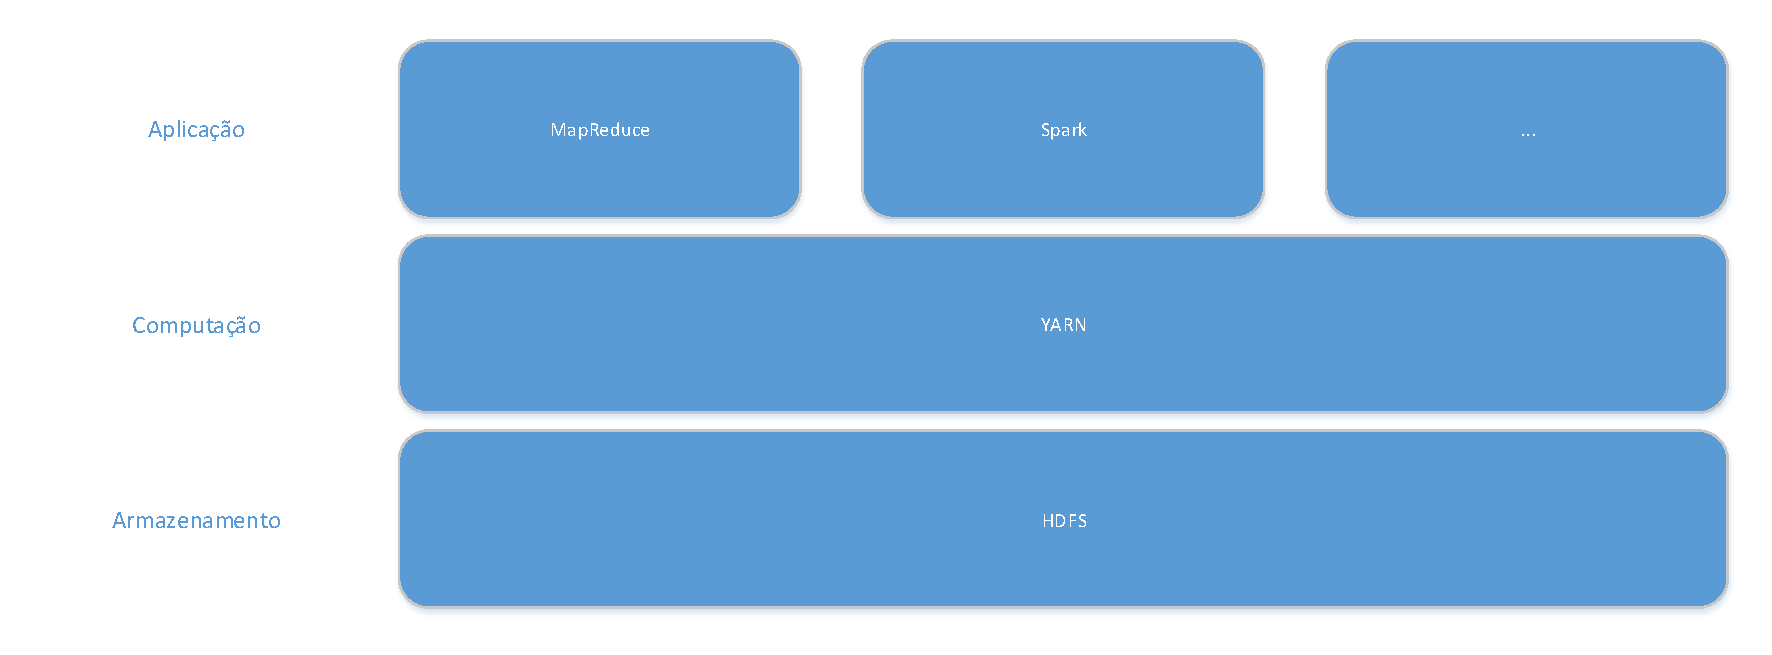
\includegraphics[width=1\textwidth]{./img/hadoop-layers.pdf}}
 \caption{Organização do Hadoop em camadas.}
 \label{fig:hadoop}
\end{figure}

A Figura \ref{fig:mrworkflow} mostra o fluxo de execução básico do MapReduce. 
A Fase de \textit{Shuffle \& Merge} não será detalhada no trabalho, mas é 
importante salientar que existe um processamento entre as fases de mapeamento e 
redução.

\begin{figure}[ht]
 \centerline{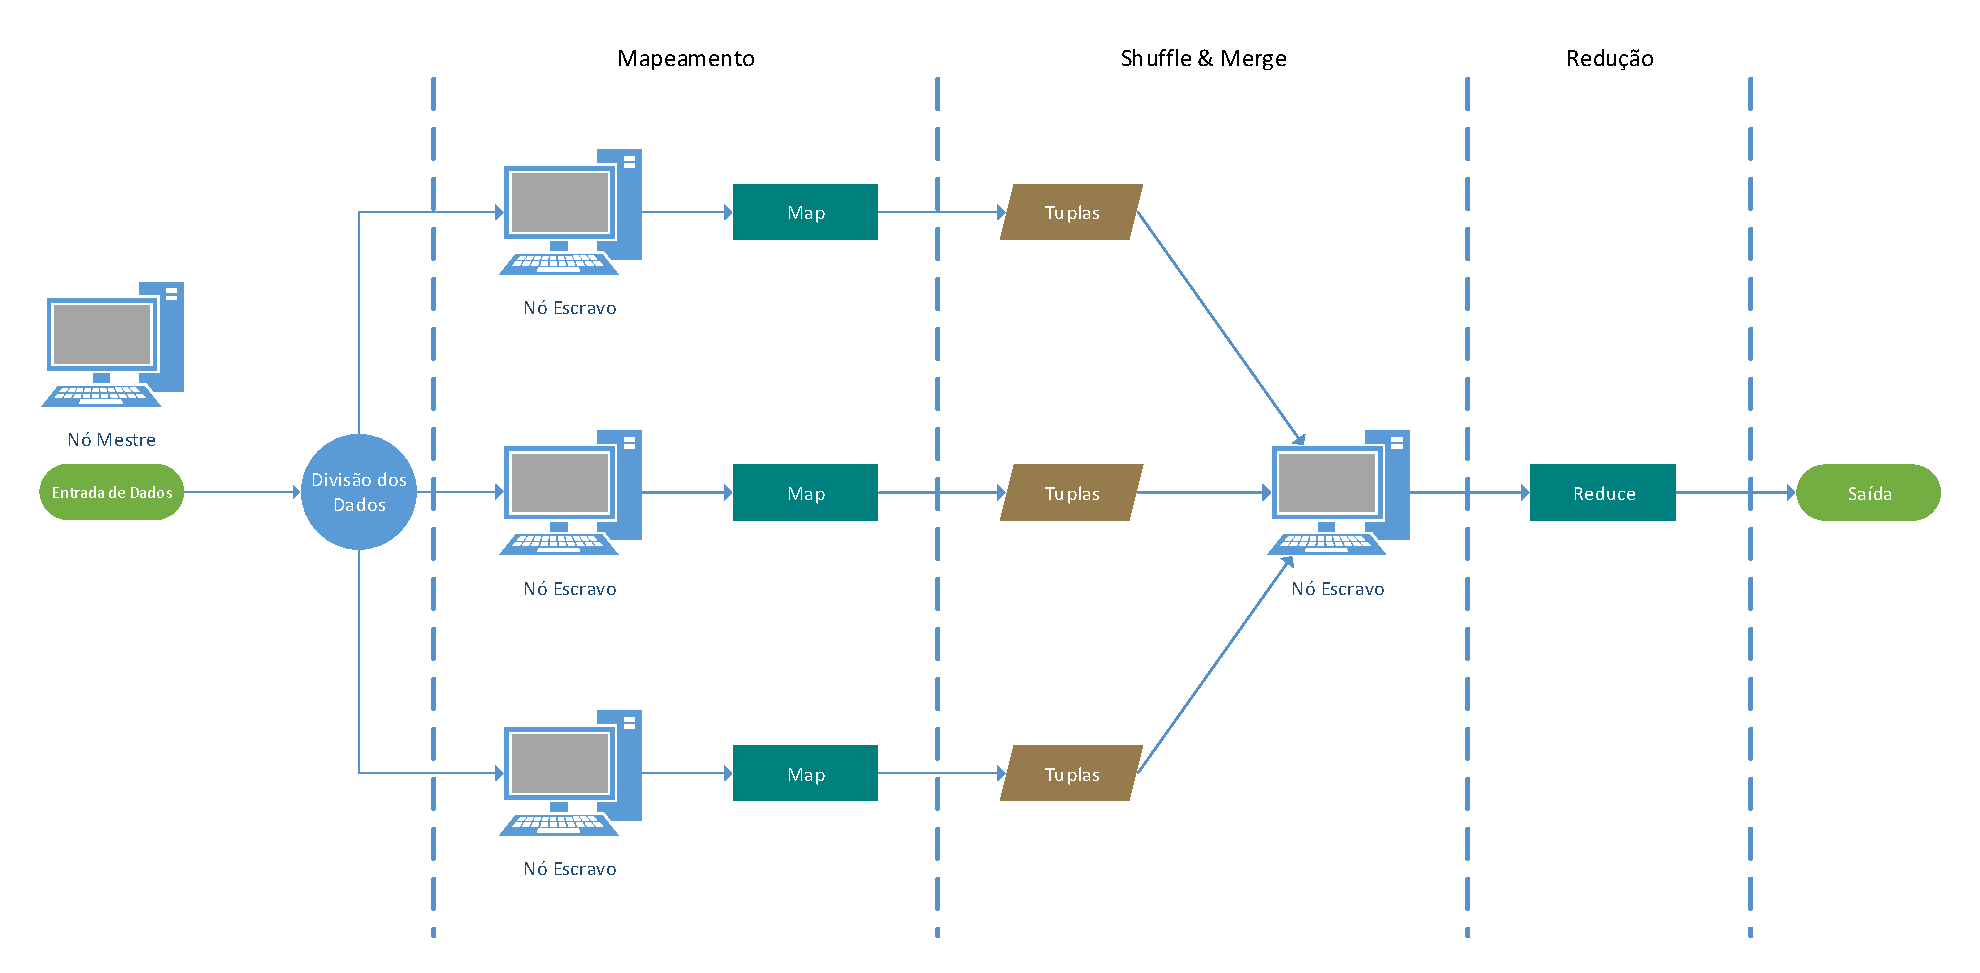
\includegraphics[width=1\textwidth]{./img/mapreduce-workflow.pdf}}
 \caption{Fluxo de execução do MapReduce.}
 \label{fig:mrworkflow}
\end{figure}

Primeiramente temos os dados sendo inseridos no Sistema de Arquivos Distribuído 
(\textit{Distributed File System} ou DFS) da plataforma. Os arquivos são 
divididos em pedaços de tamanho fixo e distribuídos sobre a plataforma. Isso 
permite que os dados sejam tratados de forma rápida pois há paralelização em sua 
leitura.

Com os dados armazenados, pode se iniciar a fase de mapeamento, que resulta em 
conjuntos de tuplas intermediárias. Estas sofrem um pré-processamento na fase 
de \textit{Shuffle} e são disponibilizados para os nós que irão executar a fase 
de redução. Finalmente, os executores da redução obtêm os dados e desempenham 
suas tarefas, gerando a saída da execução.

Voltando a Figura \ref{fig:hadoop}, na segunda camada encontra-se o gerenciador 
de recursos do arcabouço. O YARN (\textit{Yet Another Resource Negotiator}) foi 
introduzido no Hadoop 2.0 e além de melhorar a implementação do modelo 
MapReduce, suporta outros paradigmas de computação. Ele fornece APIs para 
requisitar e manipular recursos, não sendo comum o usuário interagir 
diretamente com essa camada.

Como o Hadoop trabalha sobre dados muito grandes, é comum que tais cargas de 
trabalho ultrapassem a capacidade de uma única máquina física. Isso implica na 
necessidade de particionar os dados sobre múltiplas máquinas. Os sistemas de 
arquivos que lidam com tal tipo de armazenamento são denominados sistemas de 
arquivos distribuídos. Hadoop possui sua própria implementação de um 
DFS, inspirado no \textit{Google File System} (Comumente 
referenciado como \textit{GFS}), denominado \textit{Hadoop Distributed 
Filesystem} (\textit{HDFS}), que é representado como a terceira camada da 
Figura \ref{fig:hadoop}.

De forma similar a sistemas de arquivos convencionais, é utilizada a abstração 
de blocos, que consistem no volume mínimo para leitura e escrita. Enquanto 
nestes, eles têm tipicamente poucos bytes, o tamanho de blocos no HDFS 
é na ordem de megabytes, sendo por padrão, 128 (configurável pelo usuário, por 
arquivo). Tal abstração permite ao Sistema: armazenar arquivos maiores do que 
qualquer disco no ambiente; simplifica o gerenciamento do armazenamento de 
dados; e facilita replicação para garantir alta disponibilidade.

Um HDFS possui dois tipos de nós: \textit{namenode} e \textit{datanodes}. Eles 
seguem uma política mestre-escravo, onde o nó do primeiro tipo atua como mestre 
e gerencia o sistema de arquivos e nós do segundo tipo recebem requisições (de 
clientes ou do \textit{namenode}) e armazenam ou recuperam blocos. Também é 
possível executar um \textit{secondary namenode} para evitar pontos únicos de 
falha na arquitetura. O principal papel deste nó é manter uma cópia dos dados de 
gerência do \textit{namenode} principal, em caso de falhas, ele pode assumir o 
lugar deste.

\subsection{Spark} \label{ref:spark}

Spark é um conjunto de uma \textit{engine} unificada e um conjunto de 
bibliotecas para processamento de dados distribuídos \cite{ref:sparkbook}. A 
motivação para sua criação foi a necessidade de muitos tipos de processamento e 
a tendência do ferramental ser cada vez mais específico no cenário de 
\textit{Big Data}.

A arquitetura do Spark pode ser visualizada na Figura \ref{fig:spark-arch}. A 
\textit{engine} usualmente é executada sobre um cluster de máquinas gerenciado 
por um \texttt{Gerenciador de Cluster}, que mantém o controle dos recursos 
disponíveis. Ele oferece suporte a três gerenciadores: um do próprio Spark, 
Hadoop YARN ou Mesos \cite{ref:mesos}.

\begin{figure}[ht]
 \centerline{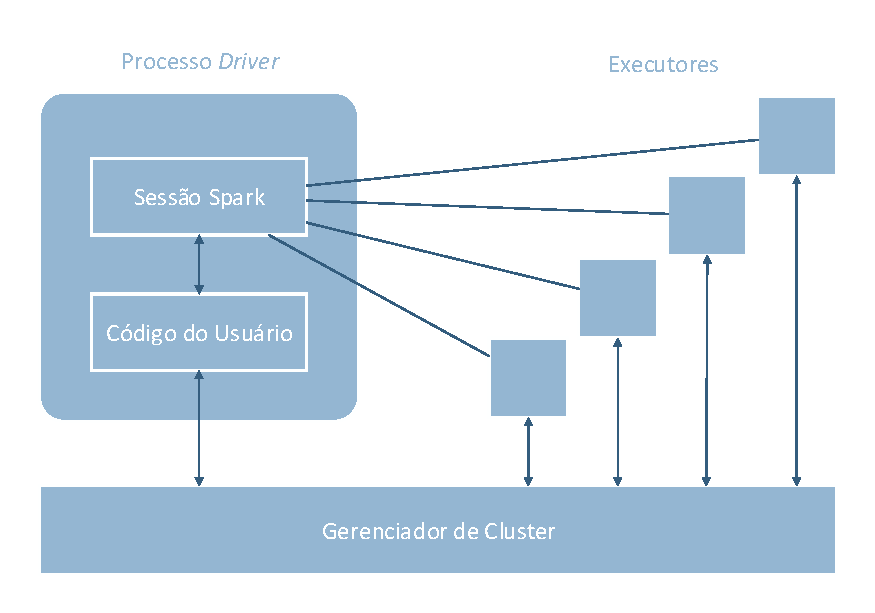
\includegraphics[width=1\textwidth]{./img/spark-arch.pdf}}
 \caption{Arquitetura de uma aplicação Spark.}
 \label{fig:spark-arch}
\end{figure}

O \texttt{Processo Driver} é responsável por manter o ciclo de vida da 
aplicação. Dentre suas responsabilidades estão: responder às entradas do 
programa do usuário; analizar, distribuir e agendar trabalho sobre os 
\texttt{Executores}; e manter informação relevante sobre a execução. Os 
\texttt{Executores} realizam duas funções: executam tarefas que lhes são 
atribuídas e reportam o estado das computações para o \texttt{Processo 
Driver}.

O Spark é atrelado a um modelo de programação similar ao MapReduce, todavia, 
possui uma abstração para compartilhamento de dados, chamada \textit{Resilient 
Distributed Datasets} (RDDs). Estas, consistem em coleções de objetos tolerantes 
a falhas e que podem ser manipulados em paralelo e são particionados sobre a 
infraestrutura que executa a engine. 

Spark manipula RDDs através de uma API unificada disponibilizada para diversas 
linguagens, que facilita o desenvolvimento de aplicações. Nela, o usuário é 
capaz de passar funções locais para serem executadas de forma distribuída. A 
avaliação dos RDDs é realizada de forma \textit{Lazy}, o que significa que as 
manipulações são efetivadas apenas quando é executada uma ação nos dados, que 
se trata de uma instrução para computar o resultado de uma série de 
transformações. Isso permite que ele encontre um plano de execução eficiente 
pois pode agregar operações, otimizando o tempo de execução.





